\documentclass[11pt]{article}
\usepackage[margin=0.78in]{geometry}
\usepackage{amsmath,amssymb,booktabs,graphicx,hyperref,microtype,xcolor}
\hypersetup{colorlinks=true,linkcolor=blue!55!black,urlcolor=blue!55!black}
\graphicspath{{figures/}{evidence/context/}}
\title{Axisymmetric Brill-wave collapse in AthenaK:\\progress, gauge controls, and outer-boundary test}
\author{Numerical investigation report}
\date{15 August 2026}

\begin{document}
\maketitle

\section{Executive status}
The calculation uses the Figure-3 Brill datum with amplitude
$A=-0.047$ and independently measured ADM mass
$M_{\rm ADM}=2.660301967997158$.  IrisK's two-dimensional single-domain
spectral representation is interpolated directly inside AthenaK; the lapse is
initialized as $\alpha=\psi^{-2}$.  The evolution is the axisymmetric Cartoon
Z4c system at nominal N128, sixth spatial order, RK4, and
\texttt{dchi\_max=0.02}.  None of the results in this report is a completed
Figure-3 reproduction or production qualification.

The strongest completed evolution remains the shock-avoiding lapse with zero
shift: it covered the full paper proper-time interval before a substantially
later failure.  Vanilla advective $1+\log$ plus a fixed-$\eta$ Gamma driver
also reached $t=20M$.  The scale-invariant telegrapher family continues to
develop late curvature and constraint growth.  The experiments below isolate
constraint damping, KO dissipation, shift choice, AMR depth, and boundary
distance without enabling a $\chi$ floor or weakening the strict-positive
prolongation gates.

\section{Initial-data port and early diagnostics}
The original M0-wiring comparison revealed patch-like structure when the
single-domain spectral datum was routed through the older domain machinery.
The accepted path instead evaluates the authenticated two-dimensional IrisK
coefficients directly on AthenaK cell centers.  Initial evolution-variable and
constraint plots were produced from AthenaK's imported fields, rather than
from an external IrisK rendering.  The initial constraints are finite; the
large late-time constraint features discussed here arise during evolution.

No apparent horizon finder is enabled in this Brill diagnostic series.  A
failure to report a horizon is therefore not evidence that a horizon is
absent.

\section{Gauge survey before the present five controls}
The first max-$|K|$ telegrapher plus max-$|K|$ Gamma-driver run failed at
$t\simeq10.163M$.  Setting Z4c $\kappa_1=\kappa_2=0$ did not extend that
lifetime and made the terminal constraints much larger.  Replacing all
max-$|K|$ coefficient normalizations by fixed coefficients delayed failure to
$t\simeq16.52M$, while changing only the shift damping from
$2\max|K|$ to fixed $\eta=2$ delayed it to $t\simeq16.74M$.  Thus runaway
shift damping was a major stiffness source, but not the only instability.

Three field-local telegrapher scales---$|K|$, $\sqrt{K_{ij}K^{ij}}$, and
$\sqrt{\gamma^{ij}\partial_i\chi\partial_j\chi}$---all failed earlier than
the domain-maximum control.  Their spatial profiles are reproduced in
Fig.~\ref{fig:mu}.  Scaling $\tau$ and $\kappa$ together from $(1,1)$ to
$(2,2)$ reduced the discrete damping stiffness while keeping wave speed
unchanged, but both level-20 evolutions failed at central proper time
$\tau\simeq10.38M$.

\begin{figure}[t]
  \centering
  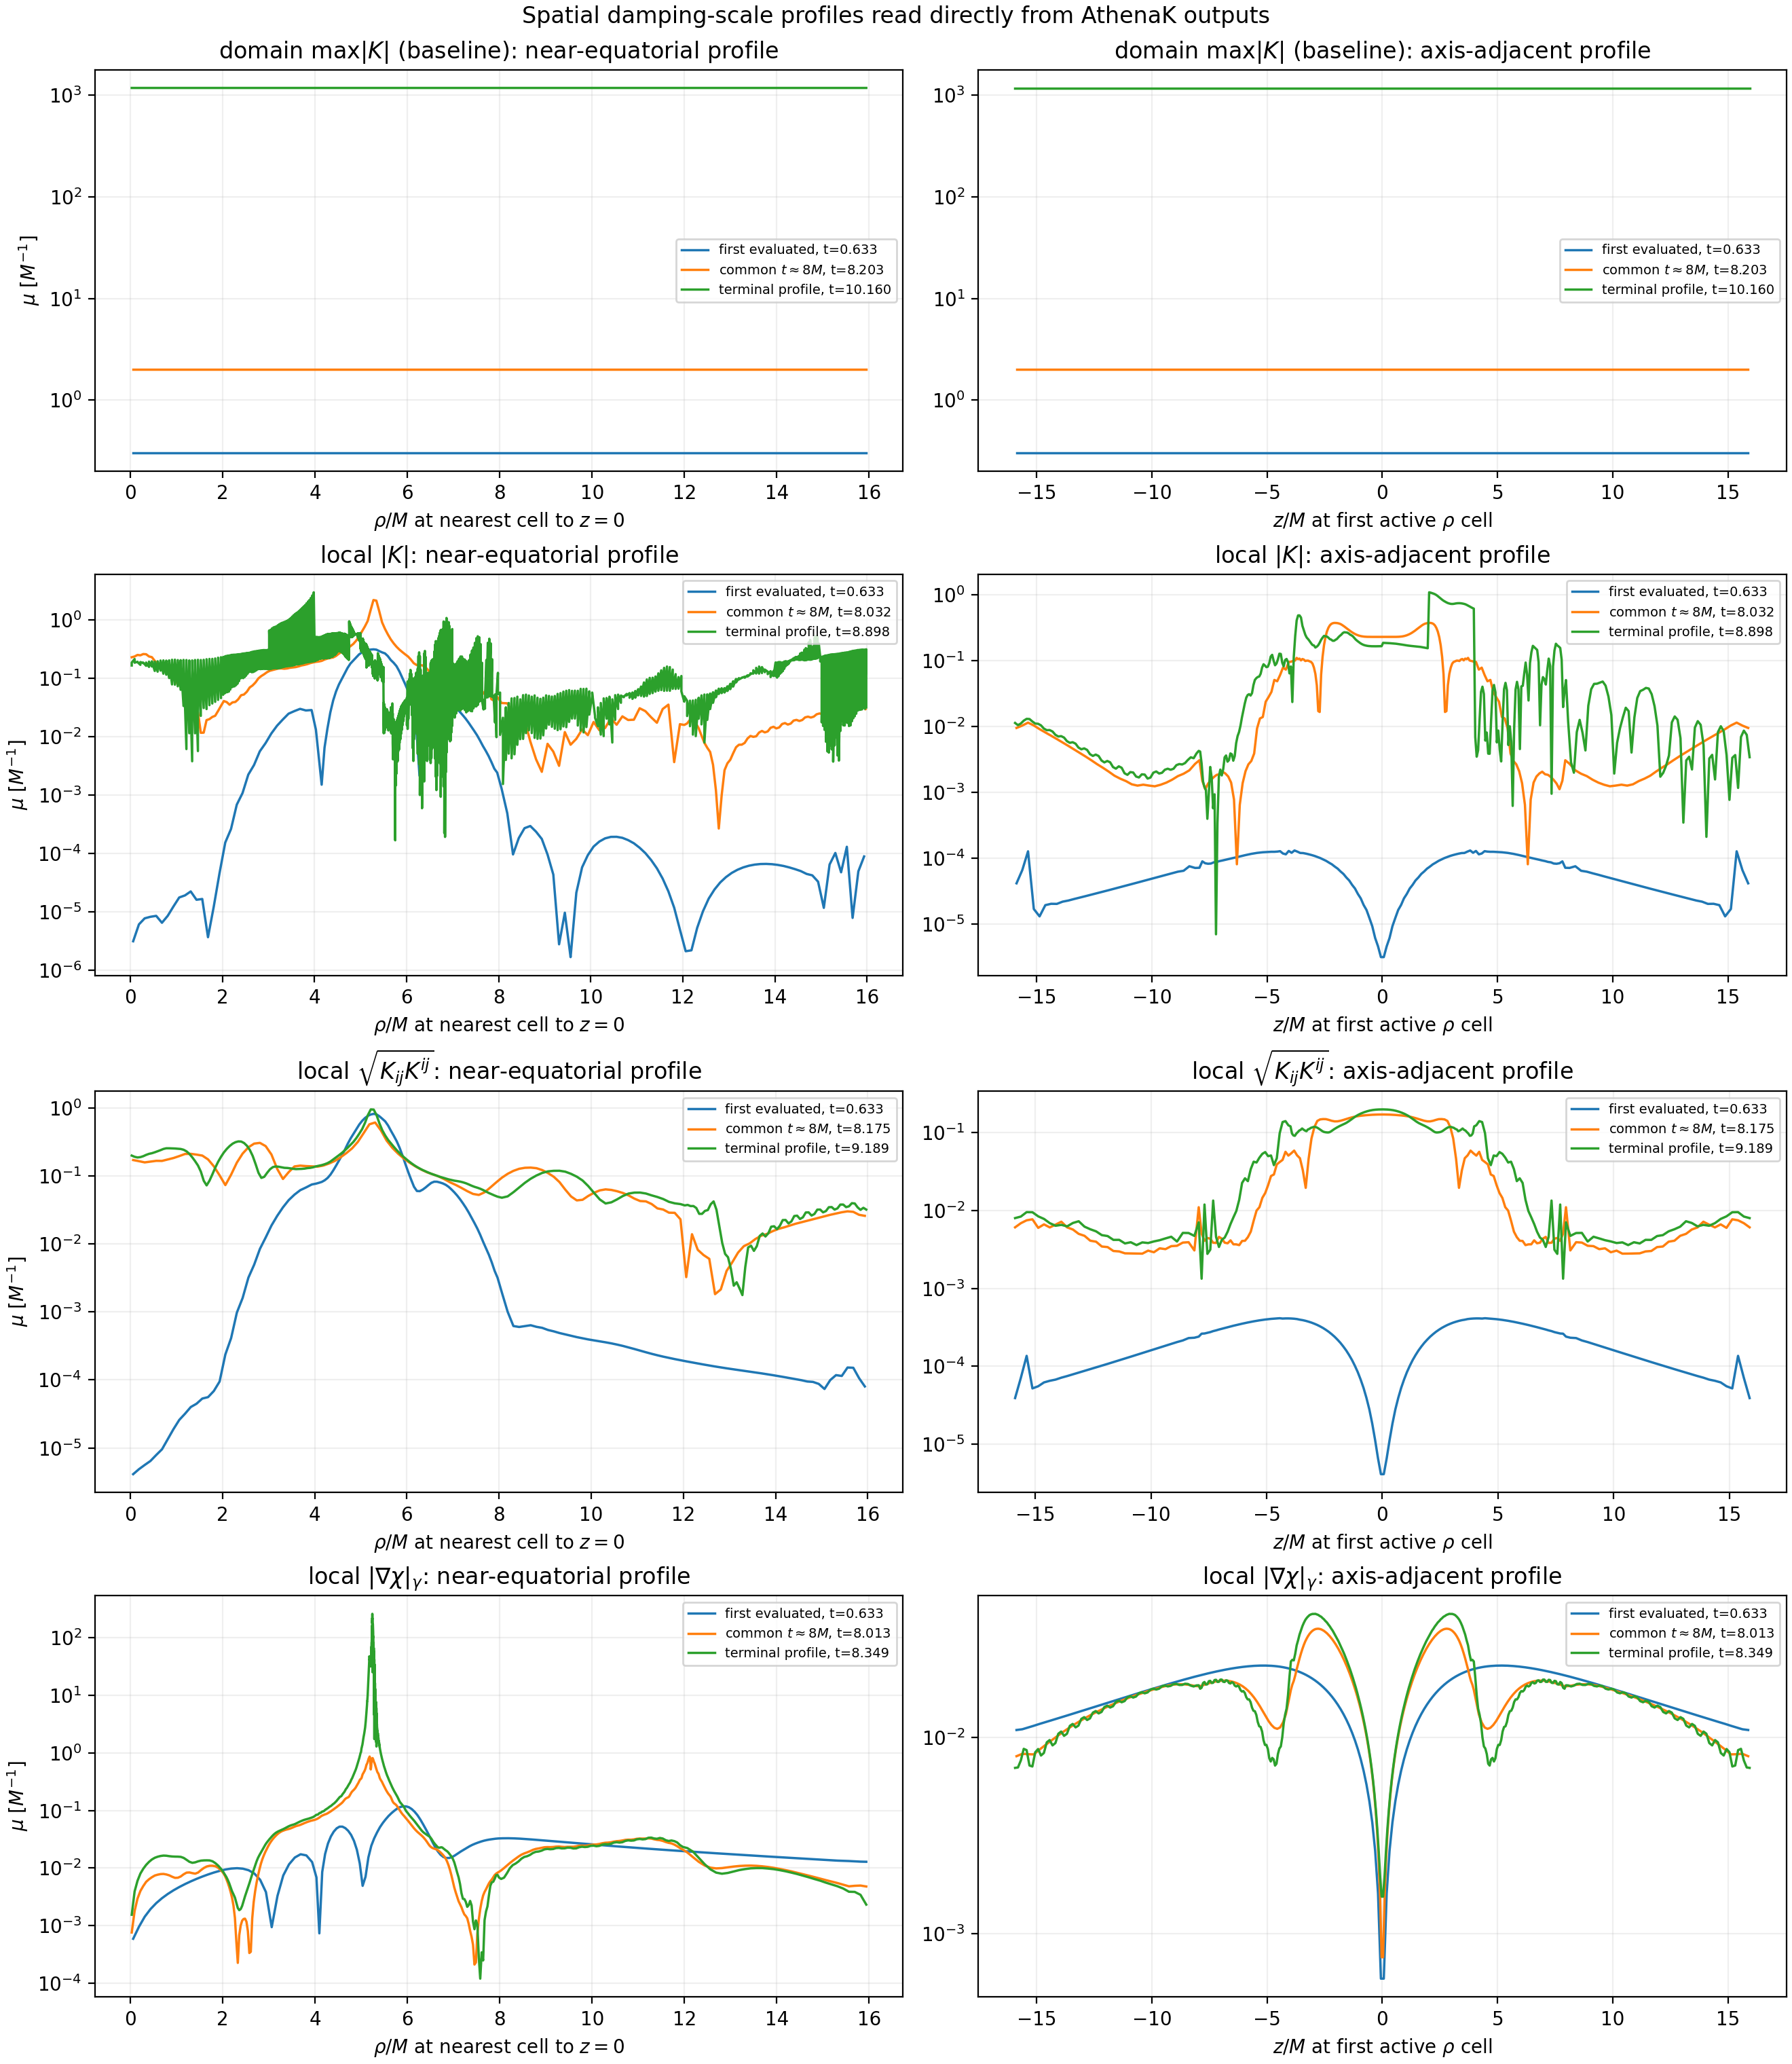
\includegraphics[width=0.96\linewidth]{telegraph_mu_spatial_profiles.png}
  \caption{Previously authenticated AthenaK spatial profiles for the tested
  telegrapher damping scales.  They are evolved AthenaK fields, not IrisK
  interpolation plots.}
  \label{fig:mu}
\end{figure}

The shock-avoiding/zero-shift and vanilla-$1+\log$/Gamma-driver comparisons
are retained in Figs.~\ref{fig:old-gauge}--\ref{fig:old-con}.  Their paper
curves are rendered-vector extractions because raw numerical Figure-3 data
were not published.

\begin{figure}[t]
  \centering
  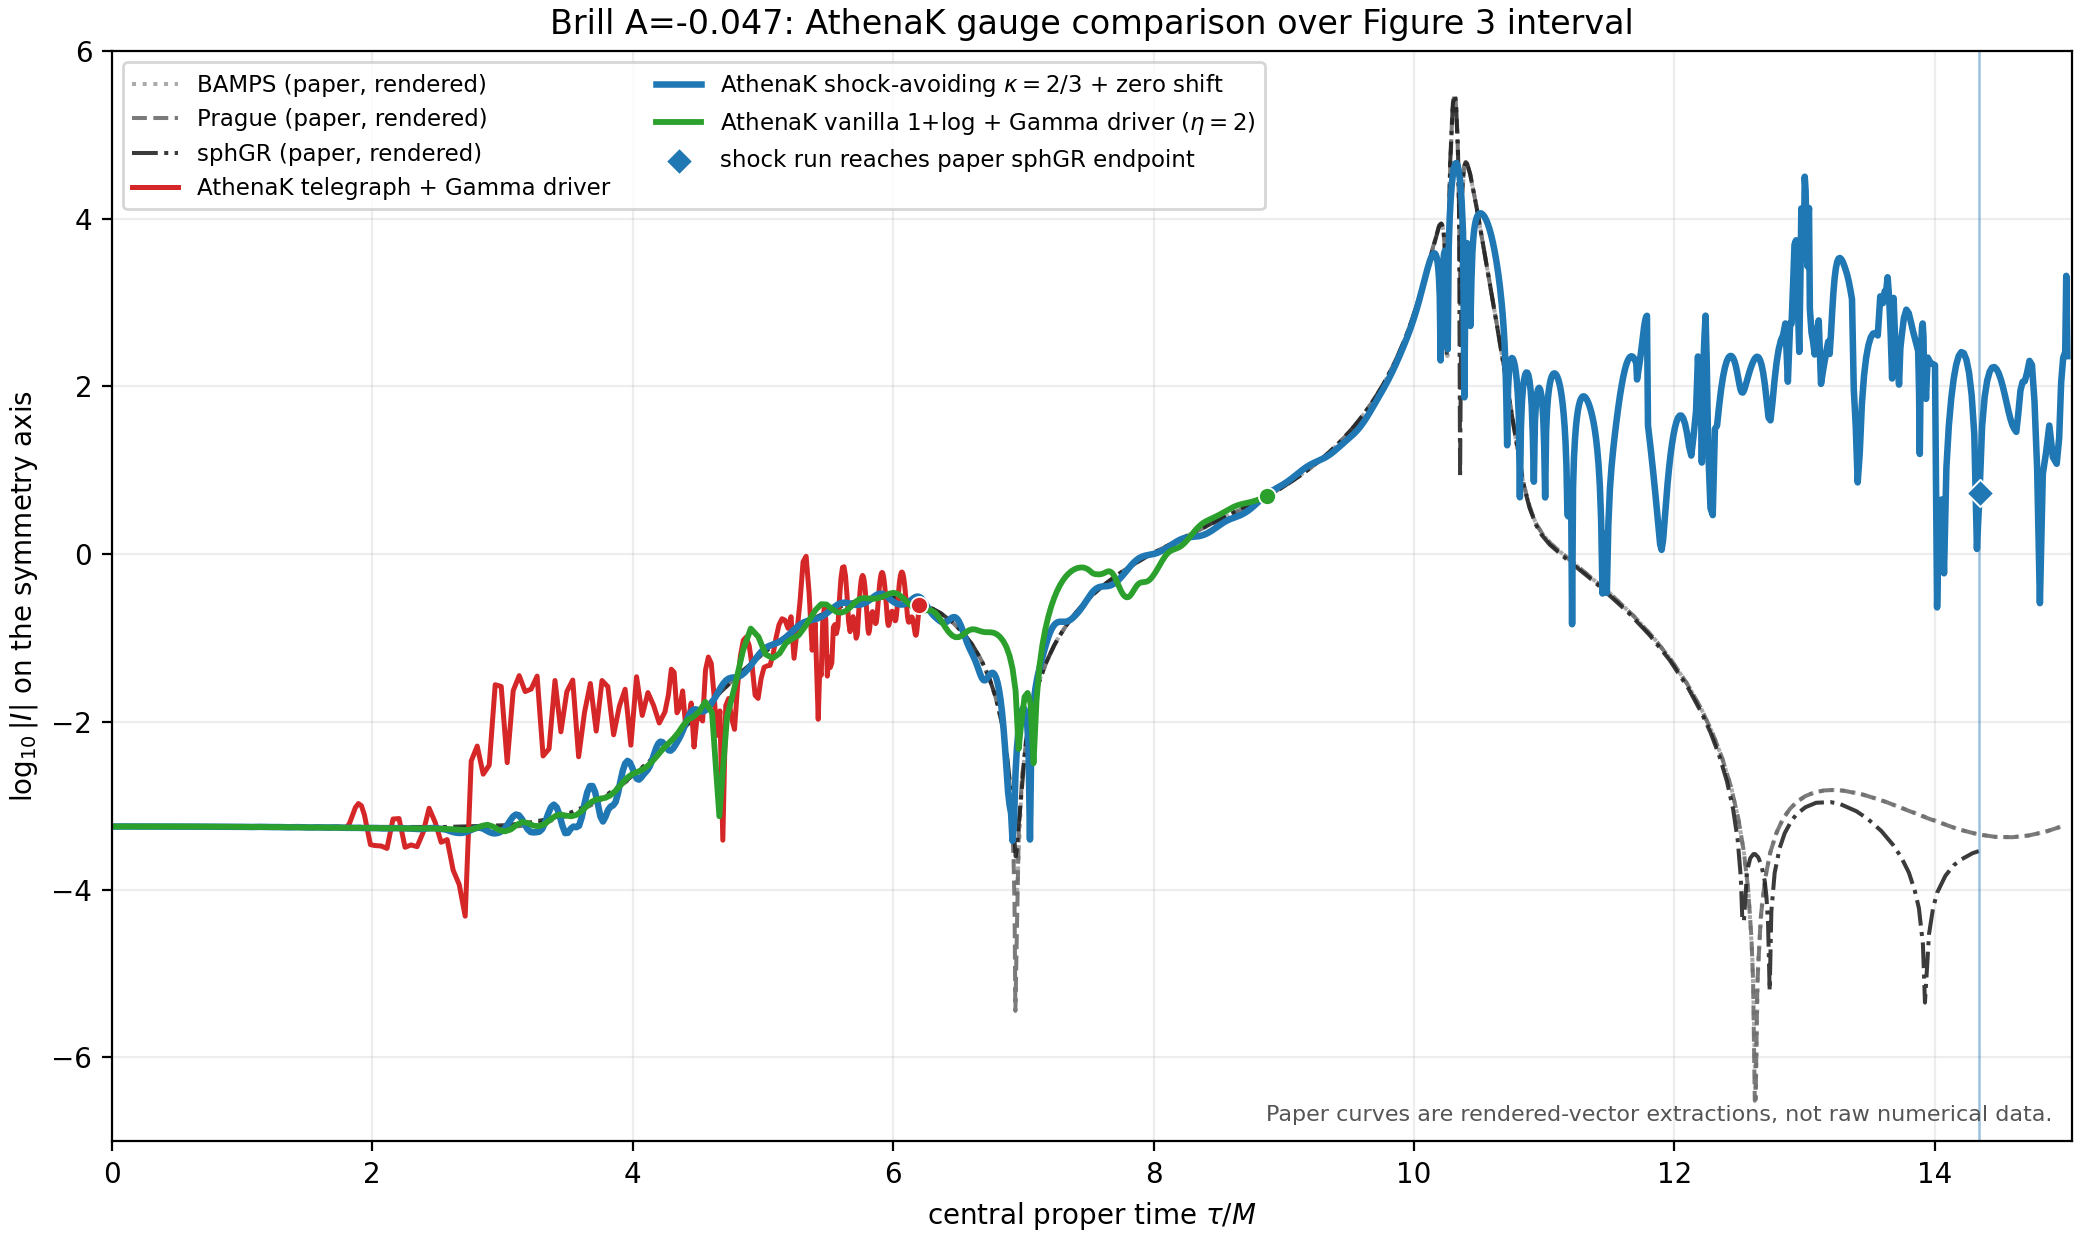
\includegraphics[width=0.93\linewidth]{figure3_extended_gauge_overlay_20260814.png}
  \caption{Earlier gauge-family overlay against the rendered Figure-3 curves.}
  \label{fig:old-gauge}
\end{figure}

\begin{figure}[t]
  \centering
  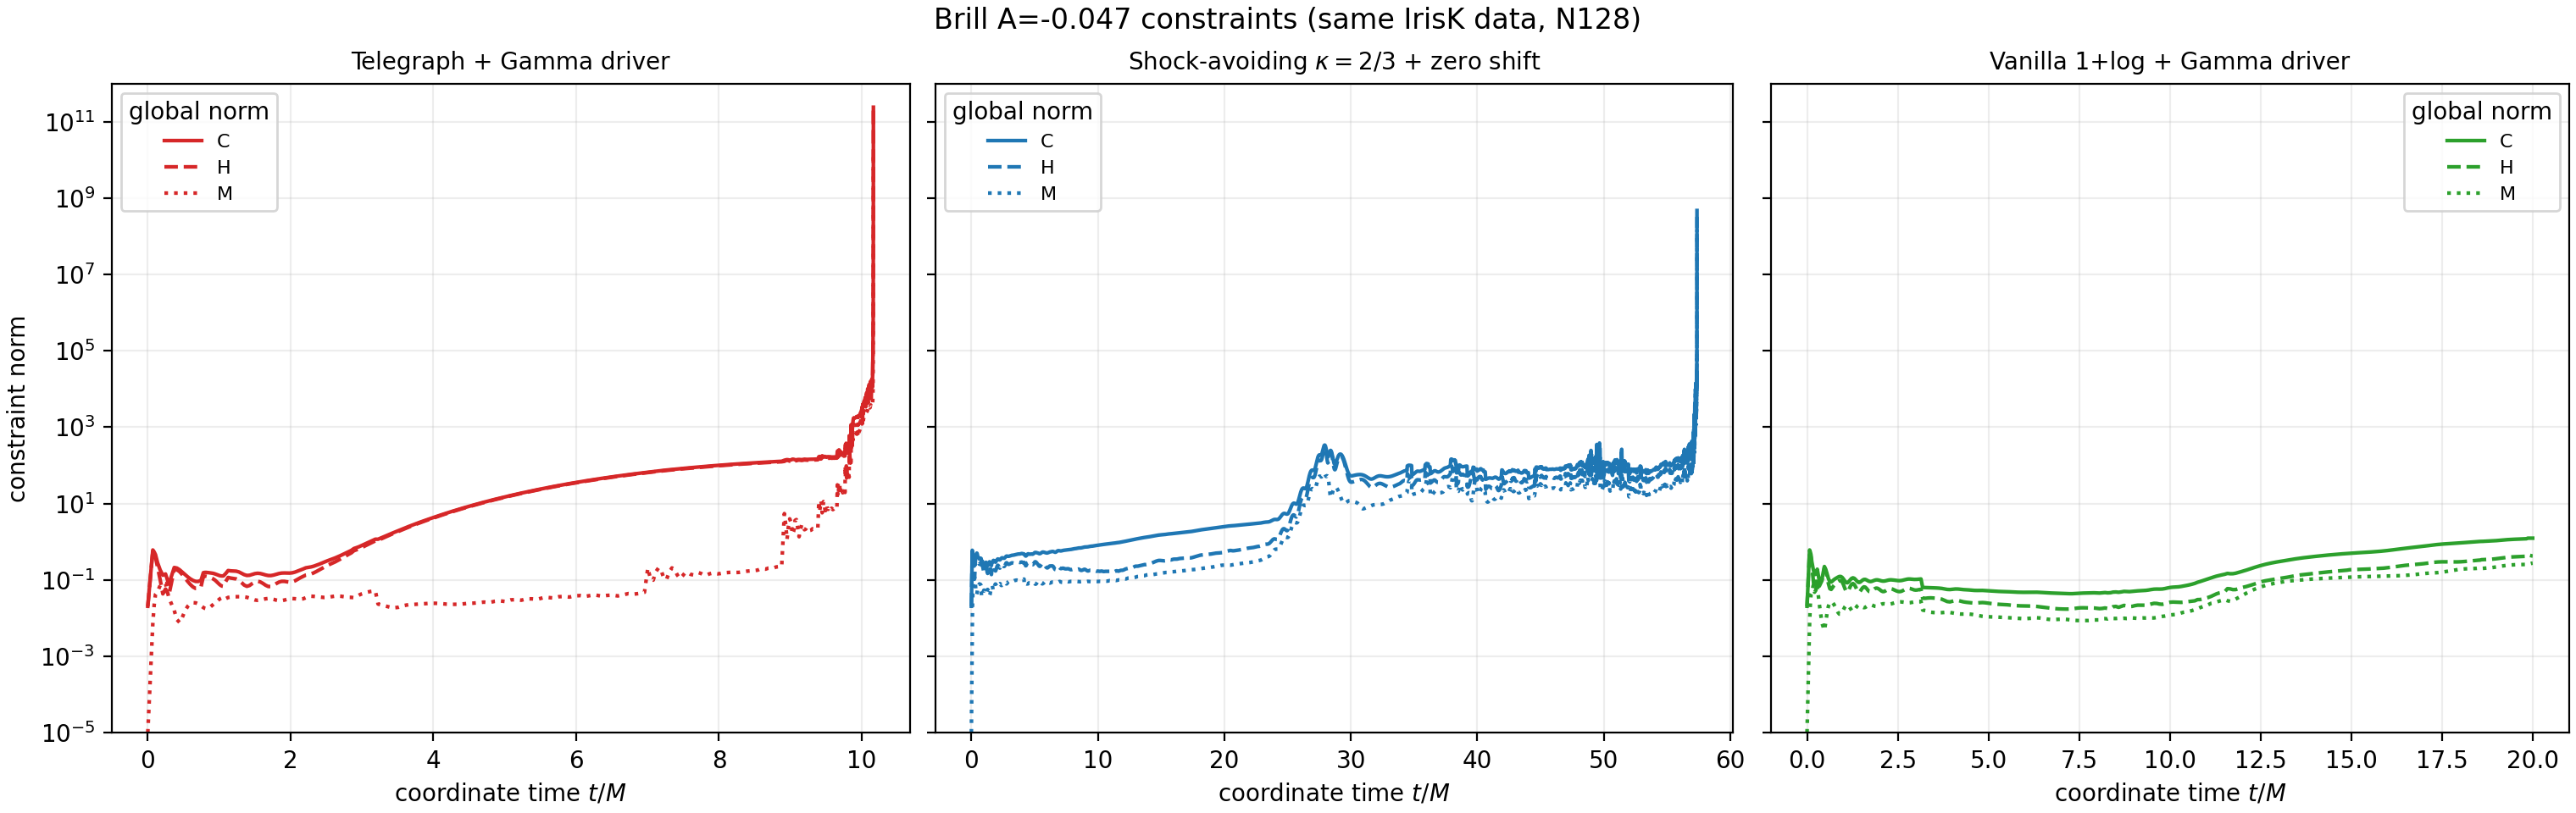
\includegraphics[width=0.93\linewidth]{constraint_extended_gauge_comparison_20260814.png}
  \caption{Earlier constraint comparison for telegrapher, shock-avoiding, and
  vanilla gauge families.}
  \label{fig:old-con}
\end{figure}

\section{Five zero-damping KO/shift/domain controls}
All five cases use the pre-collapsed telegrapher lapse, $(\tau,\kappa)=(1,1)$,
max-$|K|$ scaling, and exactly zero Z4c constraint damping.  Cases 1--3 use
$0\le\rho\le16$, $|z|\le16$.  Cases 4--5 repeat the later KO=0.5 cases on
$0\le\rho\le64$, $|z|\le64$.  The base spacing remains $0.25$ because the
root grids grow from $64\times128$ to $256\times512$; the larger-box test does
not trade boundary distance for resolution.

The original KO=0.5 cases approach the 8,192-block operational guard.  At the
user's direction, the enlarged-domain cases run sequentially on one A100 in
the shared-interactive queue.  The single-rank and global guards are therefore
both 16,384 blocks.  That capacity change is not an AMR-criterion change:
\texttt{dchi\_max=0.02} and maximum physical level 20 remain fixed.  It is
reported explicitly because an earlier capacity or GPU-memory stop is a
scaling result, not a boundary-condition diagnosis.

The first single-GPU attempt used an A100-SXM4-40GB.  Both cases imported the
IrisK data and passed the finite initial constraint conversion, but Kokkos then
failed before evolution while allocating the 4.883-GiB load-balance send
buffer.  Because the 16,384-block single-rank contract reserves paired send
and receive buffers, reducing this capacity would reintroduce the known AMR
block guard rather than test the boundary.  The strict successor therefore
kept one GPU and every science parameter unchanged while requiring an
A100-SXM4-80GB.  The five-case plots use only that successor's evolved data;
the 40-GiB attempt is retained as operational evidence, not counted as a sixth
science curve.

The 80-GiB successor ran the two enlarged-domain cases strictly one at a time.
The fixed-shift case reached its numerical endpoint in the first numbered
step.  The following zero-shift step was still evolving normally when its
per-step wall-time expired.  A fresh one-case successor therefore resumes
only that zero-shift case from its latest complete authenticated restart, on
one shared-interactive A100-SXM4-80GB.  The pre-restart and continuation
histories are joined at the restart time and plotted as one physical case;
the restart is not a sixth gauge/domain configuration.

The timestep is dynamic through the CFL/AMR controller, not through an
explicit max-$|K|$ stiffness estimate.  For this Z4c implementation the
candidate timestep is the MPI-global minimum represented cell width times
\texttt{cfl\_number=0.15}.  With base spacing $0.25$, level $L$ therefore gives
$\Delta t=0.0375/2^L$: levels 8, 9, 10, and 20 correspond respectively to
$1.46484\times10^{-4}$, $7.32422\times10^{-5}$,
$3.66211\times10^{-5}$, and $3.57628\times10^{-8}$.  The controller does not
currently insert max-$|K|$, lapse, shift, $\tau$, $\kappa$, or a measured gauge
speed into that Z4c estimate.  Hence severe wall-time growth in these runs is
directly tied to refinement depth, even when the gauge coefficients are held
fixed.

\begin{table*}[t]
\centering
\small
\begin{tabular}{rlllrrrrrl}
\toprule
case & outer $R=Z$ & shift & KO & $t_{\rm last}$ & $\tau_{\rm last}$ & $\alpha_{\rm axis}$ & $L_{\max}$ & AH & terminal \\
\midrule
1 & 16 & fixed $\eta=2$ & 0.02 & 16.722 & 10.365 & 0.64398 & 20 & no & strict positive-$\chi$ gate \\
2 & 16 & fixed $\eta=2$ & 0.5 & 16.714 & 10.372 & 0.64496 & 20 & no & exit 1 \\
3 & 16 & zero & 0.5 & 7.4926 & 4.5815 & 0.5979 & 13 & no & exit 1 \\
4 & 64 & fixed $\eta=2$ & 0.5 & 16.714 & 10.372 & 0.64496 & 20 & no & strict positive-$\chi$ gate \\
5 & 64 & zero & 0.5 & 7.4927 & 4.5816 & 0.5979 & 20 & no & strict positive-$\chi$ gate \\
\bottomrule
\end{tabular}
\caption{The five requested controls.  Last values are the last fully finite history rows, not post-failure extrapolations.  The AH column is recorded telemetry only; the horizon finder was disabled for this diagnostic series.}
\label{tab:five-cases}
\end{table*}
\paragraph{Horizon status.} No finite history row in any of the five cases reported an apparent horizon.


\begin{figure*}[t]
  \centering
  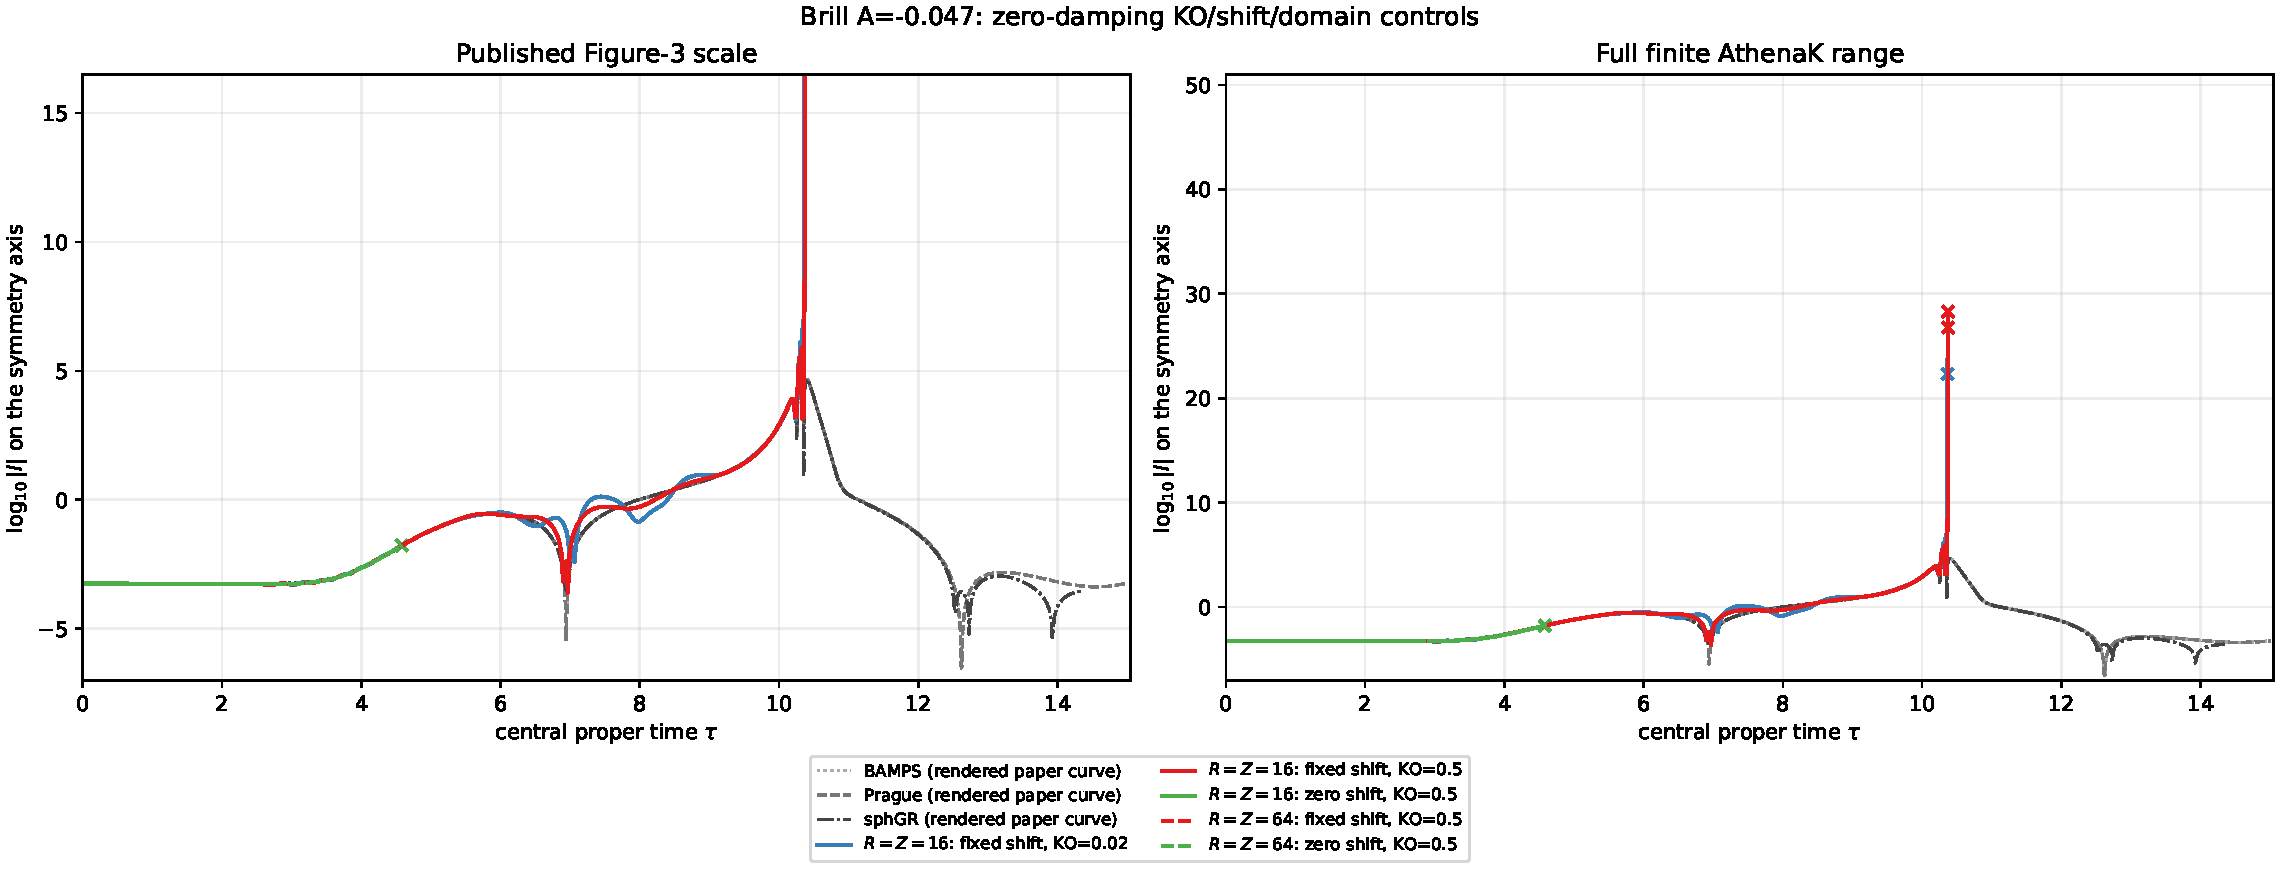
\includegraphics[width=0.98\textwidth]{figure3_five_case_overlay.pdf}
  \caption{All five requested controls overlaid on the rendered published
  Figure-3 curves.  Crosses mark each last finite AthenaK row.}
  \label{fig:five-fig3}
\end{figure*}

\begin{figure*}[t]
  \centering
  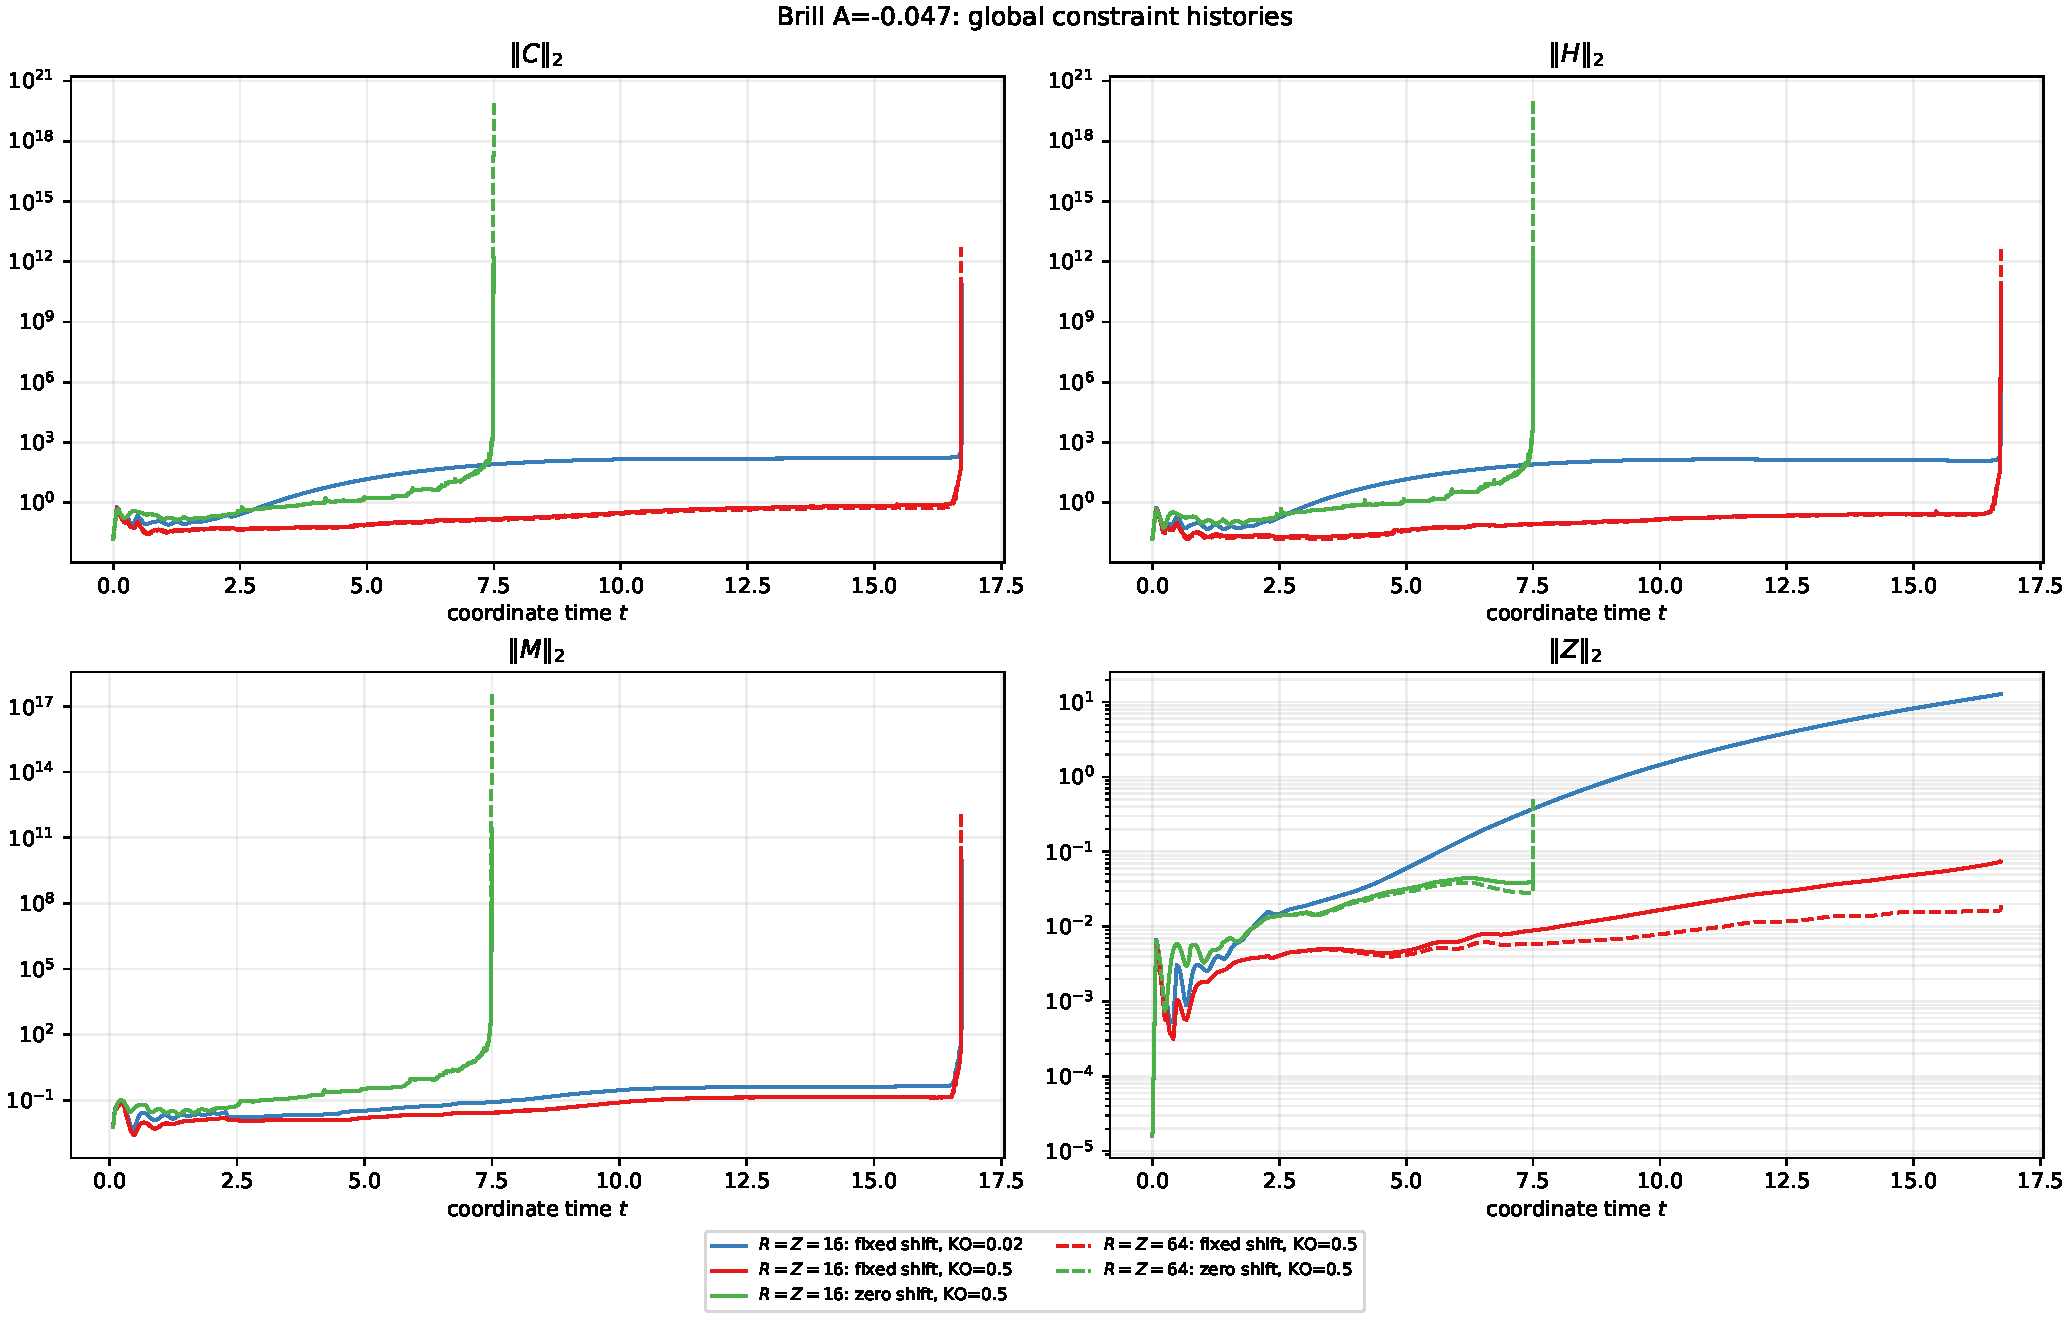
\includegraphics[width=0.98\textwidth]{constraints_five_case.pdf}
  \caption{Global Z4c constraint histories for all five controls.}
  \label{fig:five-con}
\end{figure*}

\begin{figure*}[t]
  \centering
  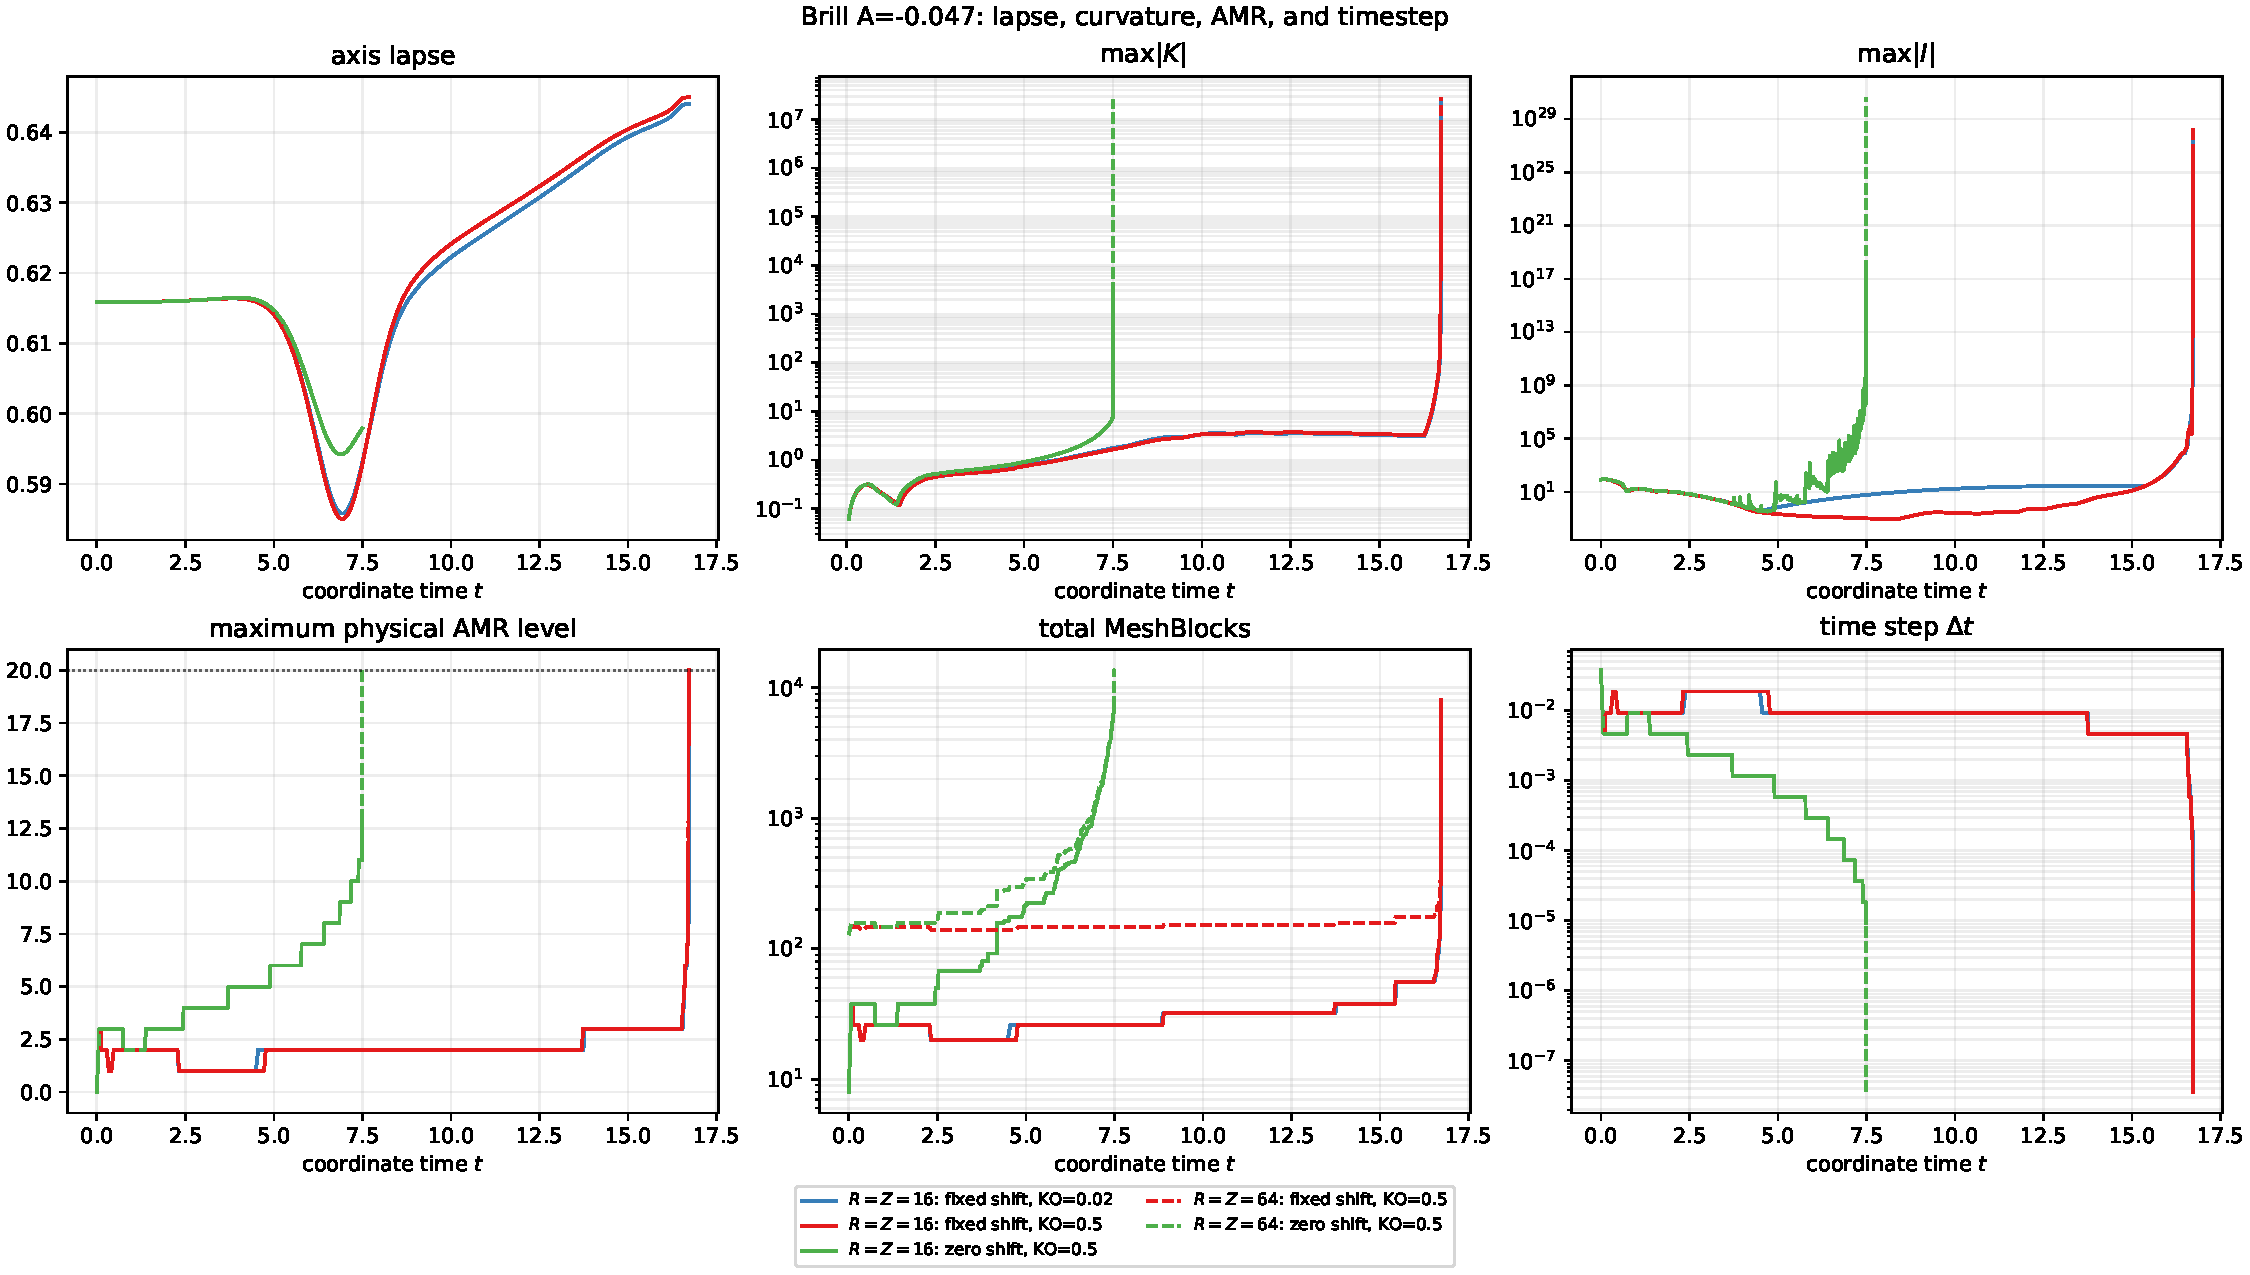
\includegraphics[width=0.98\textwidth]{gauge_amr_five_case.pdf}
  \caption{Axis lapse, curvature, AMR inventory, and timestep diagnostics.}
  \label{fig:five-amr}
\end{figure*}

\begin{figure*}[t]
  \centering
  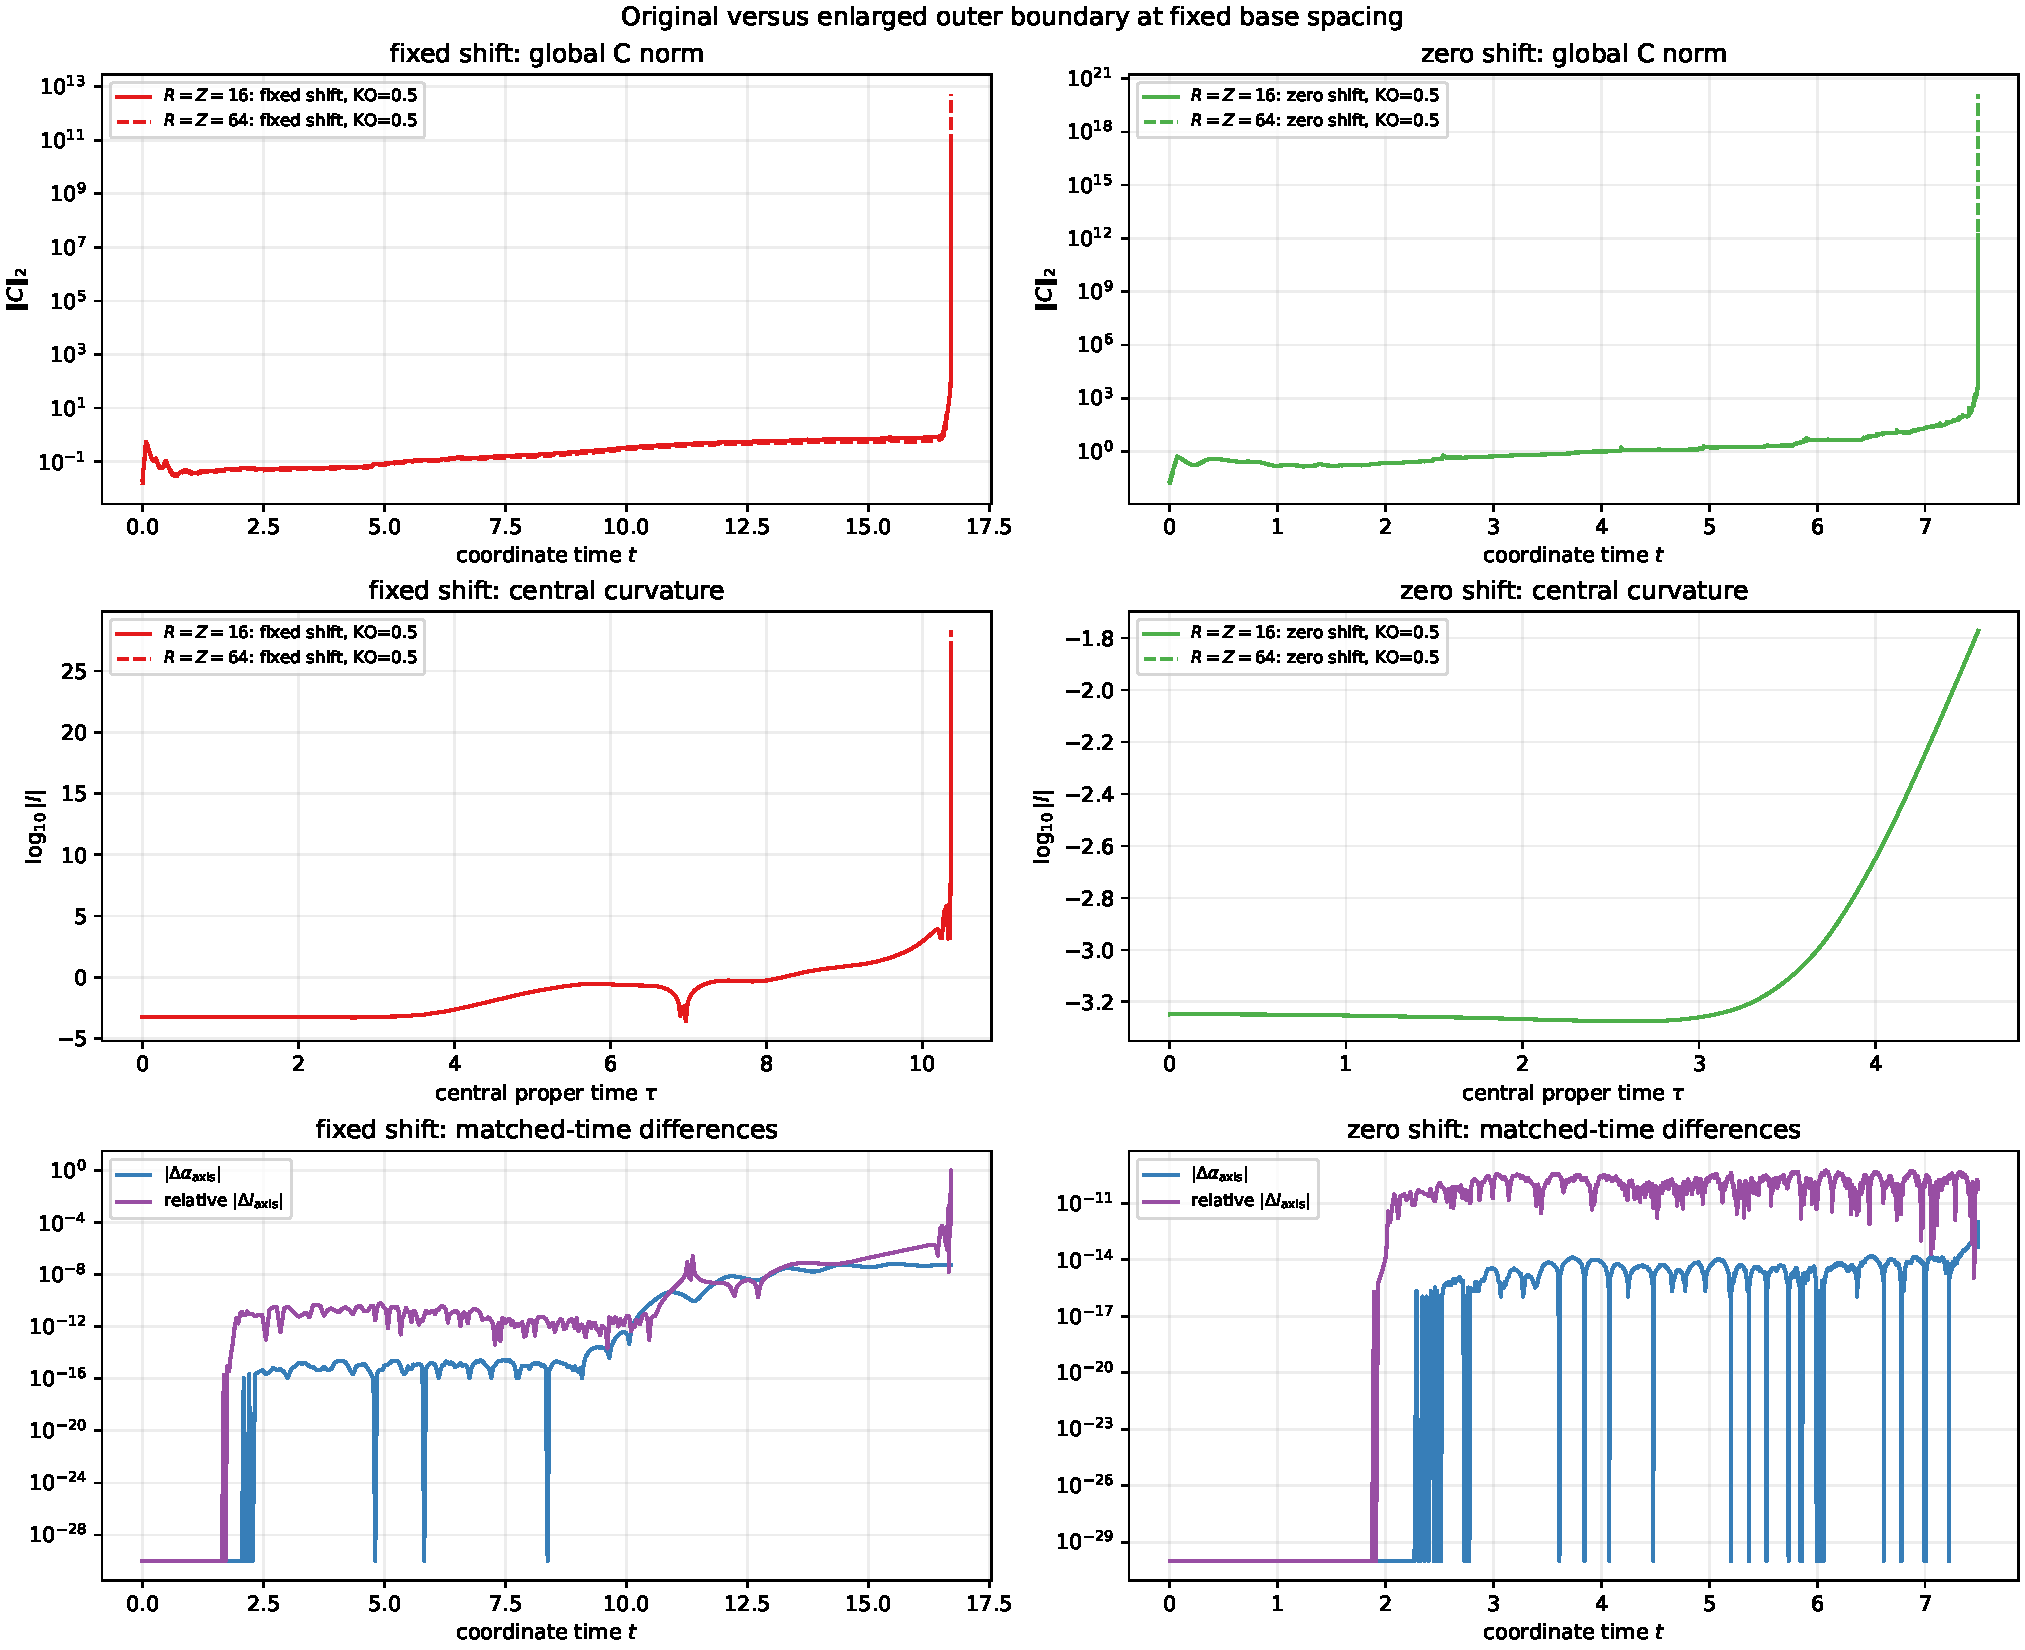
\includegraphics[width=0.98\textwidth]{boundary_distance_pairwise.pdf}
  \caption{Pairwise original-domain/enlarged-domain comparisons for the two
  KO=0.5 shift choices.  Solid and dashed lines differ in boundary distance
  while retaining the same base spacing.}
  \label{fig:boundary}
\end{figure*}

\section{Interpretation and remaining uncertainty}
The enlarged-domain runs are designed to answer a narrow causal question:
whether late artifacts move materially when the outflow boundary is causally
farther away.  Agreement before the original light-crossing time disfavors a
direct outer-boundary explanation; divergence does not by itself prove a
boundary reflection because the AMR tree can differ.  The pairwise plots and
terminal inventories must therefore be interpreted together.

For the fixed-shift KO=0.5 pair, interpolation at matched coordinate times
shows that the axis lapse agrees to better than $8\times10^{-8}$ and the
axis curvature to about $1.2\times10^{-6}$ through $t=16$.  The terminal
times are likewise essentially identical: $16.7140508$ on the original box
and $16.7140514$ on the enlarged box.  The global constraint norms differ
more because their volume integrals cover different domains, but the central
gauge and curvature histories rule out the original outer boundary as the
driver of this fixed-shift failure.  The zero-shift pair agrees even more
closely through the original box's terminal time, $t=7.4925751$.  At that
matched time the relative differences in the global $C$, $H$, and $M$ norms
are respectively $5.3\times10^{-6}$, $1.1\times10^{-5}$, and
$2.6\times10^{-5}$; max-$|K|$ differs by $1.8\times10^{-5}$ and the global
maximum curvature by $1.2\times10^{-6}$.  The axis lapse differs by only
$1.0\times10^{-12}$, central proper time by $1.3\times10^{-14}$, and axis
curvature by $7.8\times10^{-11}$ relatively.  The small $Z$ norm is more
volume-sensitive and differs by 17\%, but this does not accompany a central
trajectory difference.  The enlarged case then passes the original
8,192-block stop, reaches the configured maximum physical level 20 and 13,580
blocks, and continues to display the same catastrophic constraint/curvature
growth.  It finally stops at $t=7.4927181$ when the unchanged strict gate
rejects 2,346 nonpositive or nonfinite parent stencils for $\chi$.  The
original boundary is therefore not the cause of the zero-shift instability;
its lower capacity only selected the earlier terminal event.  The full
terminal comparison is reported in Table~\ref{tab:five-cases} and
Fig.~\ref{fig:boundary}.

The current evidence does not support curing the telegrapher evolution by
arbitrarily raising KO dissipation, enabling a $\chi$ floor, or selectively
relaxing a strict gate.  The most promising algorithmic direction remains a
smoother scale-invariant gauge scale than a domain maximum, together with
explicit history telemetry and restart-authoritative filtering.  Any such
change needs a prospective matched comparison rather than tuning to one
terminal time.

Taken together, these controls disfavor three simple explanations as the sole
cause.  The fixed and zero-shift choices both fail, although at different
times; raising KO dissipation from 0.02 to 0.5 does not remove the late growth;
and moving the outer boundary from 16 to 64 leaves the central trajectories
and terminal times essentially unchanged.  This does not prove that gauge or
dissipation is irrelevant, but it means that another blind parameter sweep is
not the most discriminating next experiment.

The cleanest prospective resolution test is to increase the cell count inside
each MeshBlock while retaining the logical root-block layout, physical domain,
maximum AMR level, $d\chi$ threshold, gauge, and KO coefficient.  This raises
the resolution at every represented level without deliberately changing the
refinement policy.  Dynamic thresholding can nevertheless produce a different
tree; therefore the run must archive physical refinement coverage and block
decisions, or use a prescribed/replayed refinement mask if literal tree
identity is required.  Pre-terminal convergence of the constraints and a
systematic delay of the terminal event with decreasing spacing would favor
under-resolution or a numerical instability.  A terminal event at nearly the
same physical time and location would instead favor a formulation/gauge
limitation.  A separate, one-factor-at-a-time matrix should vary the initial
base resolution and $d\chi_{\max}$ to measure AMR-criterion sensitivity; these
changes should not be combined in the first resolution comparison.  None of
these proposed runs was executed for this report.

\section{Reproducibility boundaries}
The final artifact binds the selected original-domain ledger, enlarged-domain
initial and continuation jobs, terminal manifests, settled accounting,
comparison JSON, histories, logs, rank bindings, plotting inputs, and derived
files by SHA-256.  Raw binary/restart hierarchies remain at their immutable
Perlmutter roots and are not silently reinterpreted.  All numerical failures
are retained.  This report makes no horizon, convergence, or complete
Figure-3 reproduction claim.

\end{document}
